% Chapter Template

\chapter{Introduction}
\label{part:Introduction}

Two of the most beautiful theories developed in the $ 20 ^{\text{th}} $ century are Quantum mechanics and General theory of relativity.
Generically, the theory of quantum mechanics is crucial in the description of phenomenon at the atomic scale, where the deviation from classical mechanics governed by Newton's law is significant.
On the other hand, general theory of relativity is important for the description astronomical phenomenon, where, again, the deviation from the Newton's law is significant.
One of the most important problem at our hand is to find a consistent framework that unifies both these theories, dubbed the problem of `quantum gravity'.

An important milestone in the quest for quantum gravity was achieved with the framework of perturbative quantum field theories.
This framework successfully combines quantum mechanics and special theory of relativity.
The breadth of this framework includes, but not limited to, the scattering of particles at the Large Hadron Collider, the description of the boiling water, exploration of the exotic phases of matter and Hawking radiation coming out of black hole.

Among all quantum field theories, there is a class of theories with enhanced symmetry when compared to the Lorentz invariance of special relativity.
This includes all the transformations of the spacetime which preserve angles between two lines, in addition to the transformations that preserve the Lorentzian length.
This class of theories is called `conformal field theories' (henceforth CFTs), the central topic of this thesis.

Conformal field theories appear in a variety of physical phenomenon.
An important class of them appear at the end of renormalization group flow.
Generically, the coupling constants in quantum field theories depend on the energy scale at which one probes the said theory, called `running coupling constant'.
This flow of the coupling constant can stop due to coincidences, at which point the theory becomes independent of the energy at which it is probed.
Precisely this independence on the energy scale leads to the enhancement of symmetries from Lorentz length invariance to scale invariance.
These `fixed points' of the flow of couplings are described by scale invariant theories.
In addition, one hypothesizes that this scale invariance is enhanced to `conformal invariance'.
Thus, these `end points of the flow' are described by CFTs.

Another context in which this class of theories appear is the criticality of the statistical physical models.
Ising models in various dimensions provide a detailed model of magnetization.
This model is exactly solved in two dimensions on the lattice.
It is also solved in four dimensions since the mean field approximation is exact.
However, in three dimensions, both these techniques fail to be tractable.
One simplification can be made in this case by considering the case of criticality.
In this case, the fluctuations becomes scale independent, and therefore amenable to be analyzed using the tools of CFT.

Yet another context where the study of CFTs is important pertains the `AdS/CFT correspondence'.
While a first principle construction of nonperturbative theory of quantum gravity, mentioned above, is still unclear, the `AdS/CFT' correspondence provides an indirect formulation of such a framework.
In its strongest form, it postulates the duality between two theories.
On one hand, there is the nonperturbative completion of certain type of string theory in asymptotically AdS backgrounds, certain highly symmetric solutions of Einstein equation.
On the other hand, there is a maximally supersymmetric and conformal invariant cousin of quantum chromodynamics.
This conformal invariant theory can be understood in the framework of CFTs, and therefore furnish \textit{a} definition of nonperturbative theory of quantum gravity.
\section*{Conformal field theories}
CFTs are a class of quantum field theories with enhanced symmetries.
Thus, they combine quantum mechanics with conformal invariance.
The central aspect of quantum mechanics is `Unitarity', which encodes the preservation of information.
This is an appropriate generalization of the Liouville theorem, which states that the number of possible physical states in a classical system can neither decrease nor increase.
In essence, the quantum generalization states that the number of possible physical states remain preserved, and therefore all the probabilities add to 1.
In particular, this means that the probability of any physical process must be between 0 and 1.
In quantum theories, the physical states are described by rays in the Hilbert space, and the corresponding probability is given by the square of the norm of the corresponding vector, as per `Born rule'.

Conformal invariance means invariance of the observables in the quantum theory under conformal transformations.
In $ d $ dimensional Euclidean space, they are encoded in the group $ SO(d+1,1) $ , as opposed to the Lorentzian theory, where it is $ SO(d,2) $.
An important class of observables in CFTs are the correlation functions of local operators, denoting the amount of correlation in the respective local operators.
These can be defined in both Euclidean and Lorentzian setup, and are related to each other via the Wightman functions.
These correlation functions depends on the types of the local operators and the respective location of these operators.
However, their form is highly constrained due to conformal invariance more than one might naively imagine.
Naively, a correlation function of $ n $ operators can be a function of $ 4n $ variables, namely, the spacetime coordinates of the $ n $ operators,
\begin{align}
  \langle  O_1\left( x_1 \right)O_2\left( x_2 \right) \dots  O_n\left( x_n \right)\rangle = f\left( x_i \right)
  .
\end{align}

Two and three points are highly constrained by conformal invariance, up to certain numbers depending on conformal representation theory.
Two point function can be written in terms of squared distances $ x_{ij}^2  = (x_i-x_j)^2 $ to be \cite{Poland:2018epd}
\begin{align}
  \langle O_{\Delta,J=0}\left( x_1 \right)O_{\Delta',J=0}\left( x_2 \right)\rangle = \frac{\delta_{\Delta,\Delta'}}{x_{12}^{2\Delta}}
  .
\end{align}

However, four point correlation functions are not fixed entirely like the two and three point case. This follows from the nontrivial dependence on the `cross ratios' \cite{Poland:2018epd}
\begin{align}
  U & =\frac{x_{12}^2x_{34}^2 }{x_{14}^2x_{32}^2 } , & V & =\frac{x_{13}^2x_{24}^2 }{x_{14}^2x_{23}^2 }
  .
\end{align}
Conformal invariance can be used to write the correlation function in terms of a function of these cross ratios by choosing some appropriate scaling behavior.
A key object in the analysis of this correlator is the `conformal block'.
It encodes the contribution of a certain exchanged primary operator and all its descendants in a single function of cross ratios.
Any Euclidean correlator can be expanded into these kinematical objects.
This allows us to separate the kinematical part of the correlation function from the dynamical part.
We will discuss these details in the next chapter.
\section*{Conformal Regge theory}

The topic of this thesis is a particular aspect of CFTs, namely, Conformal Regge theory.
The main idea is to consider certain limit of the correlation function where the dependence on the spacetime point is even more constrained which leads to more direct and analytical study of the observables of the CFTs.
This idea is rooted in the analogous simplification that occurs in the S-matrix theory, called the Regge theory.

Consider two to two scattering in a generic quantum field theory.
Conservation of momentum and Lorentz invariance forces the scattering amplitude $ A $  for such a process to be dependent on only two `Mandelstam' variables: $ s=\left( p_1 + p_2 \right)^2,\, t = \left( p_1+p_3 \right)^2 $.
Regge limit concerns the study of this amplitude in the limit large $ s $ for fixed $ t $ .
In this limit, the amplitude is expected to have a simple structure, 
\begin{align}
  A\left( s,t \right) \rightarrow s ^{\alpha\left( t \right)} f\left( t \right)
  .
\end{align}
This scaling behavior of the scattering amplitude is experimentally verified \cite{Gribov:2003nw}.

In fact, this limit provided the crucial insight to prescribe a model of meson scattering consistent with Unitarity, proposed by Veneziano.
Providing a first principle derivation of this scattering amplitude lead to the `model of dual resonances'.
This paved the way to the analysis of perturbative string theory.

Important insight from the analysis of Regge limit can be summarized in the Chew-Frautschi plot.
In this plot, one considers spin angular momentum in the $ x $ axis and squared mass in the $ y $ axis.
Then, one plots the exchanged particles in the scattering process as points in this space.
These plots from the experiments have an approximate structure of a straight line.
Thus, the idea is to consider these particles as a `Regge trajectory' rather than individual particles.
In particular, the spin quantum number is not necessarily quantized, but rather is a general complex number.

While perturbative string theory in the asymptotically flat spacetime is rather well understood, its analogue in the curved spacetime is unclear due to technical difficulties.
However, one expects a similar structure as in the flat spacetime.
To begin understanding this structure, it is useful to consider anti de-Sitter space in $ d+1 $ dimensions, since they are maximally symmetric backgrounds.

AdS/CFT correspondence \cite{Maldacena:1997re} states the equivalence of string theory in these spacetime with an independently defined CFT.
Therefore, Regge limit of string theory in AdS should reflect itself as some limit in the dual CFT description.
Two to two scattering amplitude admits a dual description in terms of the four point correlation function.
The role of the Mandelstam invariants in CFT case is played by the cross ratios.
Therefore, one considers analogous limit of the correlation functions.
As described in \cite{Costa:2012cb}, this limit can be pictured in the Lorentzian cylinder as in \cref{fig:ReggeFig}.
\begin{figure}[htbp]
  \centering
  \begin{tikzpicture}
    %draw a square with points at (2,0) (0,2) (0,-2) (-2,-2)
    \draw[thick] (4,0) -- (0,4)  -- (-4,0) -- (0,-4)-- cycle;
    %draw side bisectors
    \draw[dashed,opacity=0.4] (2,2) -- (-2,-2);
    \draw[dashed,opacity=0.4] (2,-2) -- (-2,2);
    %points
    % \node[below] at (0.7,0) {$5$};
    % \draw[fill,black](0.7,0) circle (0.05cm);
    \node[below] at (2,1.7) {$1$};
    \draw[fill,black](2,1.8) circle (0.05cm);
    \node[above] at (2,-1.8) {$3$};
    \draw[fill,black](2,-1.8) circle (0.05cm);
    \node[below] at (2,-2.2) {$4^{-}$};
    \draw[fill,gray,opacity=0.4](2,-2.2) circle (0.05cm);
    \node[above] at (-2,-1.8) {$2$};
    \draw[fill,black](-2,-1.8) circle (0.05cm);
    \node[above] at (2,2.2) {$2^{+}$};
    \draw[fill,gray,opacity=0.4](2,2.2) circle (0.05cm);
    \node[below] at (-2,1.8) {$4$};
    \draw[fill,black](-2,1.8) circle (0.05cm);

    %arrows for Regge 
    \draw[->,opacity=0.4,-latex'] (1.6,1.1) to[out=90,in=225] (2,1.7);
    \draw[->,opacity=0.4,-latex'] (-1.6,1.1) to[out=90,in=-45] (-1.9,1.7);
    \draw[->,opacity=0.4,-latex'] (1.6,-1.1) to[out=270,in=135] (1.9,-1.7);
    \draw[->,opacity=0.4,-latex'] (-1.6,-1.1) to[out=270,in=45] (-1.9,-1.7);

    \draw[opacity=0.4,thick,dashed] (4,-4) -- (4,4);
    \draw[opacity=0.4,thick,dashed] (-4,-4) -- (-4,4);
    %plot axis and label
    \draw[-stealth] (4.9,0) -- (4.9,0.5) node[anchor=south]{$ t $ };
    \draw[-stealth] (4.9,0) -- (5.4,0) node[anchor=south]{$ y $ };
  \end{tikzpicture}
  \caption{Regge limit configuration in the Lorentzian cylinder.}
  \label{fig:ReggeFig}
\end{figure}

\section*{Outline}
This sets the stage for the work in this thesis.
First, we describe the implications of the Regge theory on the CFT data extracted from one loop string theory.
While independent computation of the string theory amplitudes are available mainly in flat space and some $ AdS_3 $ backgrounds, we can employ bootstrap techniques to arrive at a subset of data in $ AdS_5 $.
We can also use the flat space string theory analysis to constrain the amplitude in $ AdS_5 $, since effectively $ AdS_5 $ acts like a one parameter extension of flat space background.

In the latter part, we discuss the generalization of the Conformal Regge theory to many point correlation functions.
We first review the case of multi-Regge limit in the many particle scattering amplitude in quantum field theories.
Then, we discuss its generalization to the conformal field theories.


\section{Kinematics of conformal field theory}
Now, we turn to a detailed introduction of the theories considered in this thesis.

In this section, we discuss the kinematics of conformal field theory.
Conformal field theories in $ d $ dimensions are a class of quantum field theories with additional symmetries that are not present in the standard quantum field theories.
In the Euclidean space, the conformal field theories are invariant under the Euclidean conformal group, $ SO(d+1,1) $, while in the Lorentzian space they are invariant under the Lorentzian conformal group, $ SO(d,2) $.
The generators of the Euclidean conformal group can be written in terms of the spacetime derivative $ \partial_{\mu} $ as
\begin{align}
  \text{Translations}                      &  & P_{\mu} & = \partial_{\mu}                                                            ,  \\
  \text{Rotations}                         &  & M_{\mu} & =  i\left( x_\mu \partial_\nu - x_\nu \partial_\mu \right)                   , \\
  \text{Dilatations}                       &  & D       & = i x^\nu \partial_\nu                                                       , \\
  \text{Special conformal transformations} &  & K_{\mu} & = i\left( 2x_\mu \left( x^\nu \partial_\nu \right) -x^2 \partial_\mu \right)
  .
\end{align}
However, some of these generators act nonlinearly on the spacetime points.
Therefore, it is useful to consider `Embedding space':
\begin{align}
  X^A = \left( \frac{1+x^2}{2},\frac{1-x^2}{2},x^\mu  \right)  ,
\end{align}
with the signature $ \left( -,+,\dots,+ \right) $.
The Euclidean conformal group acts linearly on $ X $.
This simplifies several calculations, for instance, the inner product in the physical space given by  $ \left( x_\mu -y_\mu \right) \left( x_\nu - y_\nu \right) \delta^{\mu\nu} $ becomes $ X\cdot Y =X_A Y_B \eta^{A B} $.
Here, $ X,Y $ are respective embedding coordinates for $ x,y $.
This allows us to identify the dependence on the spacetime variables of the correlations functions.

The physical observables in conformal field theory are the correlation functions of the local operators in the theory.
The local operators are characterized by quantum numbers of the generators of the conformal group.
We consider a special set of operators, called `primary' operators.
They are precisely the operators which are annihilated by special conformal transformations $ K_\mu O =0 $.
All the other operators are `descendants' of one of these operators, namely, they are of the form: $ \left( P_\mu \right)^n O $.
In particular, the operators are labeled by the quantum numbers for dilatations: $ \Delta $  and rotations: $ \lambda $, a Young tableux diagram for the representation.
Thus, a representation of the conformal group $ R $ is labeled by $ \left( \Delta,\lambda \right) $.
In the simple case of symmetric traceless representation, $ \lambda $ can be replaced by the number of boxes in $ \lambda $, representing the spin.

Two and three points correlation functions of the primary scalars, the primary operators with spin $ 0 $ and scaling dimensions $ \Delta_i $ can be written in terms of the embedding space as follows \cite{Poland:2018epd},
\begin{align}
  \langle\phi\left( X \right) \phi\left( Y \right) \rangle                      & =\frac{\delta_{\Delta_1 \Delta_2}}{\left( X \cdot Y \right)^{\Delta_1}} ,                                                        \\
  \langle\phi\left( X \right) \phi\left( Y \right)\phi\left( Z \right)  \rangle & =\frac{c}{\left( X \cdot Y \right)^{\alpha_{123}}\left( Y \cdot Z \right)^{\alpha_{231}}\left( Z \cdot X \right)^{\alpha_{132}}}
  .
\end{align}
We have chosen the normalization of the operators such that the two point function numerators are $ 1 $.
The numerator in the three point function, $ c $,  is called `operator product expansion coefficient' (OPE coefficient).
We have also used $ \alpha_{ijk} = \left( \Delta_i + \Delta_j - \Delta_k \right)/2 $ .

The set of representations $ R $'s of the local primary operators and their respective OPE coefficients $ c_{R_1,R_2, R_3} $ consitute a useful characterization of the observables in conformal field theory, called `\emph{CFT data}'.

While it is easy to see that the spactime dependence of the two and three point functions are fixed by the conformal invariance, the situation changes for higher point functions.
The four point function is not fixed by the conformal invariance because there exist conformal invariant `cross ratios'
\begin{align}
  U=\frac{X_{12} X_{34}}{X_{13} X_{24}}, \,\, & V= \frac{X_{14}X_{23}}{X_{13}X_{24}}.
  \label{eq:crossRatios}
\end{align}
The dependence on these cross ratios can not  be fixed by conformal invariance alone.
This allows us to write the four point correlation function of identical scalars as
\begin{align}
  \langle\phi\left( X_1 \right) \phi\left( X_2 \right)\phi\left( X_3 \right) \phi\left( X_4 \right) \rangle = \frac{1}{X_{12}^\Delta X_{34}^\Delta} A\left( U,V \right).
\end{align}
$ A $ denotes an unknown function of cross ratios.
However, since the operators $ \phi $'s are identical, their correlation function is permutation invariant.
It is easy to see that this leads to a constraint on $ A $, namely \cite{Poland:2018epd}
\begin{align}
  A\left( U,V \right) \left( \frac{V}{U} 	 \right)^\Delta & = A\left( V,U \right) .
\end{align}
This is called as the `\emph{crossing constraint}'.

The goal of conformal bootstrap is to use the consistency conditions of the conformal field theory to constrain the CFT data.
In particular, we use consistency of the four point function to arrive at constraint on the lower point functions.

In conformal field theories, one can use `\emph{operator product expansion}'.
\begin{align}
  \phi\left( x \right) \phi\left( y \right) = \sum_{\textit{primary } O} c_{\phi \phi O}\left( x-y,\partial_{x-y} \right) O\left( y \right)	.
\end{align}
Unlike a generic quantum field theory, this expansion has a finite radius of convergence.
This is an operator level statement and therefore is valid in all correlation functions.
In particular, it can be used to write down a four point correlation function in terms of the lower point correlation function.
\begin{align}
  \langle\phi\left( x \right) \phi \left( y \right)\times \phi \dots \phi \rangle &
  = \sum_{\textit{primary } O} c_{\phi \phi O}\left( x-y,\partial_{x-y} \right) \langle O\left( y \right) \phi \dots \phi\rangle	.
\end{align}
Note that the right hand side correlation function has fewer operator insertions than the left hand side correlation function.

In this thesis, we will concern outselves with unitary quantum field theories.
Unitarity of conformal field theory, which is also a quantum field theory imposes constraint on the CFT data.
This leads to a nontrivial constraint on the four point correlation function when expanded in terms of the lower point correlation functions.

These constraints are used in the program of Euclidean conformal bootstrap.
However, in this thesis, we are mainly concerned with the constraints coming from the Lorentzian consistency of the conformal field theory.
In the following, we discuss the necessary tools to discuss correlation function in the Lorentzian setup and its relation to the Euclidean correlation function.


\section{Wightman functions}
In this section, we discuss the Wightman functions and their properties.
The Wightman functions are useful in going back and forth between the properties of Lorentzian correlators and their Euclidean counterparts.
We closely follow the discussion in \cite{Hartman:2015lfa}.

For concreteness, we consider the correlation function of four identical scalars $ \phi $.
First, we discuss the Euclidean correlation function in the Euclidean space with time direction denoted by $ \tau $ and space directions labelled by $ y_i $.
As discussed before, such a correlation function is fixed up a function, $ A $, of two cross ratios $ U,V $.
We define a rewriting of the cross ratios $ U  = z \bar{z}$ and $ V = \left( 1-z \right) \left( 1-\bar{z} \right) $.
This rewriting is especially useful when we use the conformal symmetry to fix three out of the four points to be at $ 0,1,\infty $.
The point that is not fixed can be brought to the same plane as the other three points by a conformal transformation.
The location of this point is precisely $ z $ in the complex plane $i \tau + y $ .
We choose the second point to be written in terms of $ z $.
Thus, the Euclidean correlation function is given by $ A\left( z,\bar{z}=z^* \right) $.
Note that in the Euclidean setup, we have $ \bar{z} = z^* $, since $ \tau $ is real.
Now, we would like to discuss the procedure to convert this correlation function to a Lorentzian correlation function.
In this case, the Euclidean time becomes purely imaginary.
Therefore, $ z,\bar{z} $ are no longer complex conjugates of each other, but are in fact complex numbers.

In the Lorentzian setup, commutator of two operators spacelike separated.
\begin{align}
  \left[ O_1\left( x_1 \right),O_2\left( x_2 \right) \right] = 0 &  & x_1 \approx x_2.
\end{align}
In particular, if we move the point $ x_2 $ from the region spacelike separated from $ x_1 $ to the region timelike separated from $ x_1 $, the commutator encounters a jump.
This jump is reminiscant of branch cut behaviour.
In fact, the correlation function in the Lorentzian setup is given by an appropriate analytic continuation of the Euclidean correlation function.
One expects that the function $ A $ admits a branch cut when two of the points in the correlation function become lightlike separated.

We study the correlation function by first starting in the Euclidean setup with points fixed at
\begin{align}
  x_1 & = \left( 0,0,\dots,0 \right), & x_2 & = \left( \tau_2,y_2,\dots,0 \right), \nonumber \\
  x_3 & = \left( 0,1,\dots,0 \right), & x_4 & = \left( 0,\infty,\dots,0 \right)
  .
\end{align}
Now, the idea is to move the second point away from the Euclidean space positions to Lorentzian space positions.
This involves a Wick rotation $ \tau \rightarrow i t $ with appropriate $ i\epsilon $ prescription.
While doing so, one can encounter a branch cut due to the presence of the lightcones in the Lorentzian spacetime.
It is easy to see that the location of the branch cuts in $ \tau_2 $ is as depicted in figure \ref{fig:cutsInTau}.
Going from Euclidean to Lorentzian, the value of $ \tau_2 $ goes from a real number to a purely imaginary number.

One can study the implications of this branch cuts on the correlation function as a function of the cross ratios.
This branch cuts implies a branch cut in the correlation function at $ z,\bar{z} \in \left( 1,\infty \right)  $.

\begin{figure}[t]
  \centering
  \begin{tikzpicture}
    %name
    \draw[] (-5.2,3) -- (-5.2,2.5) -- (-5.7,2.5);
    \node[left] at (-5.2,2.8) {$\tau_2$};
    %axis
    \draw[->,opacity=0.3,-latex'] (0,0) -- (-5,0);
    \draw[->,opacity=0.3,-latex'] (0,0) -- (0,3);
    \draw[->,opacity=0.3,-latex'] (0,0) -- (0,-3);
    \draw[->,opacity=0.3,-latex'] (0,0) -- (5,0);
    %drawing points 
    \draw[fill=black] (0,1) circle (0.05);
    \draw[fill=black] (0,2) circle (0.05);
    \draw[fill=black] (0,-1) circle (0.05);
    \draw[fill=black] (0,-2) circle (0.05);
    %labelling
    \node[left] at (-0.4,1) {$i(y_2-y_1)$};
    \node[right] at (0,2) {$i(y_3-y_2)$};

    \node[left] at (0,-2) {$-i(y_3-y_2)$};
    \node[left] at (0,-1) {$-i(y_2-y_1)$};
    %drawing cuts
    \draw[red,opacity=0.8,dashed] (0,1) -- (-0.3,3);
    \draw[red,opacity=0.8,dashed] (0,2) -- (-0.3,4);

    \draw[red,opacity=0.8,dashed] (0,-2) -- (0.3,-4);
    \draw[red,opacity=0.8,dashed] (0,-1) -- (0.3,-3);
    \draw[black,opacity=0.8] (3,0) -- (-0.3,0.5);
    \draw[black,opacity=0.8] (3,0) -- (0,2) -- (-0.3,0.5);
  \end{tikzpicture}
  \caption{Location of cuts in the complex $\tau$ plane.
    The grey lines are the possible path, with or without crossing the branch cuts.}
  \label{fig:cutsInTau}
\end{figure}

This exotic branch structure allows us to probe more constraints on the correlation function.
In particular, there are constraints coming from the Lorentzian consistency which are hard to see from the Euclidean CFT understanding.
Euclidean correlation functions are simplified in the `OPE limit', when two of the points are colliding.
This is a somewhat singular limit, but allows us to study the correlation function analytically.
This corresponds to $ z \rightarrow 0,1 \text{ or }  \infty $ limit in the correlation function $ A $.
The complicated structure of cuts allows us access to a bigger set of singular structure of the correlation function.
We can choose to cross some of these branch cuts \emph{before} taking the limit $ z \rightarrow 0,1 \text{ or }  \infty $.
Study of such limits of the correlation function is called `Regge theory'.

An important aspect of this limit is that we access the sheets of the correlator which are not principal.
Principal sheet corresponds to the Euclidean configurations.
However, we can use many paths to go away from this region.
For instance, consider the configuration of the correlation function when $ 2 > 3  $ and $ 1 < 4 $ whereas all the other pairs are spacelike separated.
This allows us to reach the following Wightman functions,
\begin{align}
   & \langle \phi\left( x_4 \right)\phi\left( x_1 \right)\phi\left( x_2 \right)\phi\left( x_3 \right) \rangle, \nonumber \\
   & \langle \phi\left( x_4 \right)\phi\left( x_1 \right)\phi\left( x_3 \right)\phi\left( x_2 \right) \rangle, \nonumber \\
   & \langle \phi\left( x_1 \right)\phi\left( x_4 \right)\phi\left( x_2 \right)\phi\left( x_3 \right) \rangle, \nonumber \\
   & \langle \phi\left( x_1 \right)\phi\left( x_4 \right)\phi\left( x_3 \right)\phi\left( x_2 \right) \rangle
  .\end{align}
It is easy to see that in this configuration, $ 1,2 $ OPE converges on the right vacuum in the second Wightman function as $ 1 $ can be commuted with $ 3 $.
Similarly, it converges on the left vacuum in the third Wightman function since $ 2 $ and $ 4 $ are spacelike separated.
However, the first and the fourth Wightman functions do not have a convergent $ 1,2 $ OPE.
Therefore, they can not be arrived at by naive analytic continuation of the Euclidean correlation function without encountering monodromy.
One can track the path in the cross ratio space $ z,\bar{z} $ during this analytic continuation of $ x_i $.
It amounts to taking $ \bar{z} $ going across the cut $ \bar{z} = 1 $ in the clockwisek or counterclockwise direction, for the fourth and the first Wightman function, respectively.
Thus, these Wightman functions are $ A^\circlearrowleft,A,A,A^\circlearrowright $, respectively.

These four Wightman functions can be combined to write an interesting quantity, $ \text{dDisc} $.
This quantity serves as a generalization of imaginary part of the scattering amplitude, in a sense that it is manifestly positive.
It is also an important quantity since the analogue of the inversion formula feeds on it.
Formally, it is defined as
\begin{align}
  \text{dDisc} A \left( z,\bar{z} \right)  =
  \cos \left( \pi\left( a+b \right) \right) A \left( z,\bar{z} \right)
  -\frac{1}{2}\left[
  e^{i\pi \left( a+b \right)}A^{\circlearrowright}\left( z,\bar{z} \right)
  +e^{i\pi \left( a+b \right)} A^{\circlearrowleft}\left( z,\bar{z} \right)
  \right]
  .\end{align}
Here, we have used $ a = \frac{\Delta_2 - \Delta_1  }{2}, \, b = \frac{\Delta_3 - \Delta_4 }{2}$.
The phase factors come from changing the time ordering of the unequal operators.
For equal scalars, the phase factors become $ 1 $.
Incidently, this quantity also admits an elegent formulation in terms of `double commutator',
\begin{align}
  \langle \left[ \phi_1, \phi_4 \right] \left[ \phi_2,\phi_3  \right]\rangle & =
  x_{12}^{-2\Delta_\phi}
  x_{34}^{-2\Delta_\phi}
  \text{dDisc}\left( A \right)
  .\end{align}







\section{Regge theory}
We discuss some aspects of Regge theory in this section.
Regge theory concerns the study of the correlation function in the `Regge limit'.
This is a generalization of the `Regge limit' in the scattering amplitudes, which concerns the high energy limit.

Consider the case of two to two scattering amplitudes.
They are described in terms of the momenta of the external particles, $p_1, p_2, p_3, p_4$.
However, due to conservation of momenta as well as Lorentz invariance of the theory, they depend only on the two invariants, $s =-\left( p_1 + p_2 \right)^2$ and $ t =-\left( p_1 + p_3 \right)^2 $.
Regge limit concerns an extreme high energy scattering limit wherein $ s $ is large while $ t $ is fixed.

Analogously, the correlation functions of four operators in a Lorentzian conformal field theory depend on two cross ratios, $ U,V $, defined in equation \ref{eq:crossRatios}.
In terms of these cross ratios, one can consider various limits.
One can consider the `OPE limit' where two of the four operators approach each other.
This amounts to $ U \rightarrow 0, V \rightarrow 1 $ with $ \left( V-1 \right)/\sqrt{U} $ fixed.
The latter, $ \xi $, is the analogue of the scattering angle in the S-matrix case.
One can also consider the limit where one of the operators approach the lightcone of the other.
This is called the `lightcone limit'.
This amounts to $ U\rightarrow 0 $ for any $ V $.

In the Regge limit, we are concerned with a certain generalization of the OPE limit.
As described in the previous section, the correlation function has interesting analytic structure.
Therefore, one has a lot more freedom to consider the generalization of the lightcone limit.
Several lightcones of the form $ x_{ij}^2 = 0 $ are related to nontrivial analytic structure such as branch points and branch cuts in terms of the cross ratio space $ U,V $.
Regge limit concerns the OPE limit, however, it is taken after crossing the cuts in $ V $ cross ratio at $ V = 1 $.

In the following, we study the effect of this limit on the correlation function of four operators, $ \phi $.
Using conformal symmetry, we first represent the correlation function in terms of the cross ratios, $ A\left( U,V \right) $.
It admits an expansion in terms of certain kinematical functions of cross ratios called `conformal blocks', denoted by $ G $.
\begin{align}
  A\left( U,V \right) & = \displaystyle\sum_{O} \lambda_{\phi \phi O}^2 G_{O}\left( U,V \right)
\end{align}
These objects are defined for each primary $ O $ and come from summing over all the descendants of a given primary $ O $.
Each primary is a representation of the Euclidean conformal group, and therefore labeled by scaling dimensions, $ \Delta $ and the representation of the rotation group, $ \Lambda $.
For the symmetric traceless representation of the rotation group, it is just the spin quantum number.
While these are interesting objects themselves, it is useful to rewrite the expansion in terms of `conformal partial waves', $ F_{O} $.
Similar to the S-matrix partial waves, these partial waves have a well defined orthogonality properties.
They can be expressed as a linear combination of the conformal block as follows
\begin{align}
  F_{O} = G_O + \frac{\kappa_{\tilde{O} }}{ \kappa_{O}} G_{\tilde{O}}
  .\end{align}
The expressions for $ \kappa $ can be found in \cite{Costa:2012cb}.
The orthogonality holds for the operators on the `principle series representations'.
These are operators whose scaling dimensions is $ \nu = d/2 + i \mathbb{R} $.
The orthogonality relation can be written in terms of some weight function $ \mu $ as \cite{Caron-Huot:2017vep}
\begin{align}
  \int dU dV \, \mu\left( U,V \right) F_{O}\left(U,V \right) F_{O'}\left(U,V \right) = n_{O} \delta_{O \, O'}
  .
\end{align}

Since these partial waves form a complete basis, we can consider the partial wave expansion in spacetime dimensions $ d = 2 h $ \cite{Costa:2012cb, Caron-Huot:2017vep},
\begin{align}
  A\left( U,V \right) & = \displaystyle\sum_{J} \displaystyle\int_{h+ i \mathbb{R}}
  \frac{
    d\nu}{2\pi i }
  b_{\nu,J} F_{\nu,J}\left( U,V \right).                                                    
\end{align}
Here, we have introduced the `OPE function' $ b_{\nu,J} $
\begin{align}
  b_{\nu,J}           & =\frac{ \lambda_{\phi \phi O}^2}{\nu^2 - \left( \Delta-h \right)^2}
.\end{align}
It is an analytic function of $ \nu $ with poles at the location of the physical operators.

We discuss the analytic structure of the correlation function in the Regge limit as a function of $ V $.
The lightcones result in two branch point singularities at $ V = 1 $ and $ V= \infty $.
To separate them, we write a decomposition of the correlator \cite{Costa:2012cb} as follows
\begin{align}
  A & =
  A^{+} +
  A^{-}
  ,\end{align}
such that the first one has no nontrivial monodromy around $ V =1  $, whereas the later has no nontrivial monodromy around $ V= \infty $.
Corresponding to each, we define the `signatured OPE function', $ A^{\theta = \pm} $.
They are the coefficient of the partial wave expansion of the signatured correlator
\begin{align}
  A^{\theta }\left( U,V \right) & = \displaystyle\sum_{J} \displaystyle\int_{h+ i \mathbb{R}}
  \frac{
    d\nu}{2\pi i }
  b_{\nu,J}^{\theta} F_{\nu,J}\left( U,V \right)
  .
\end{align}
They get contributions from even and odd spins, respectively.
It is now known that these `signatured OPE functions' are also analytic functions of $ J $ \cite{Caron-Huot:2017vep}.
Thus, even and odd spins form `Regge trajectories'.
These are interesting analytic manifolds with analyticity in $ J $.

First, we discuss the limiting behaviour of the conformal partial wave in the Regge limit.
This limit can be written as $ \sigma \rightarrow 0 $ with fixed $ \xi  $ where we use
\begin{align}
  \sigma^2 = z \bar{z}, \, &  & \xi =
  \frac{1}{2} \left(
  \sqrt{\frac{z}{\bar{z}}} + \sqrt{\frac{\bar{z}}{z}}
  \right)
  .\end{align}
As we will discuss later in the thesis, the Regge limit of the partial wave in generic dimensions is $ \sigma^{1-J}  $.
Thus, the leading contribution to the correlator comes from the operators with higher spins.
However, operators with arbitrarily large spin appear in the spectrum.
To make sense of this sum over spins, we use the techniques from complex analysis.


We will use the analyticity in spin in the following.
We discuss the evaluation of the correlator in the Regge limit described above.
First, we replace the sum over spins by a contour integral over the positive real line, shown in blue in \cref{fig:polesInJ}.
Then, we consider deforming this contour to the red contour.
In the process, we pick any pole that we may encounter \cite{Costa:2012cb}.
This pole is called `the pomeron'.
Furthermore, the integral over $ \nu $ can also be performed in the saddle point approximation in certain cases \cite{Costa:2017twz}.
Thus, the leading behaviour of the correlator in the Regge limit is given by $ \sigma^{1-j^{*}}  $, where $ j^{*} $ is the location of the circled pole in \cref{fig:polesInJ}  evaluated at the saddle point in the $ \nu $ integral.


\begin{figure}[t]
  \centering

  \resizebox{0.6\textwidth}{!}{
    \begin{tikzpicture}
      %name
      \draw[] (-1.2,3) -- (-1.2,2.5) -- (-1.7,2.5);
      \node[left] at (-1.2,2.8) {$J$};
      %axis
      \draw[->,opacity=0.3,-latex'] (0,0) -- (-1.5,0);
      \draw[->,opacity=0.3,-latex'] (0,0) -- (0,3);
      \draw[->,opacity=0.3,-latex'] (0,0) -- (0,-3);
      \draw[->,opacity=0.3,-latex'] (0,0) -- (5.8,0);
      %drawing points 
      \draw[fill=black] (0,0) circle (0.05);
      \draw[fill=black] (1,0) circle (0.05);
      \draw[fill=black] (2,0) circle (0.05);
      \draw[fill=black] (3,0) circle (0.05);
      \draw[fill=black] (4,0) circle (0.05);
      \draw[fill=black] (5,0) circle (0.05);
      \draw[fill=black] (0.3,1) circle (0.05);

      %drawing circles
      \draw[<-,line width=0.7,blue] (0.2,0) to[out=90,in=0] (0,0.2) to[out=180,in=90] (-0.2,0) to[out=-90,in=180] (0,-0.2) to[out=0,in=-90] (0.2,0);
      \draw[<-,line width=0.7,blue] (1.2,0) to[out=90,in=0] (1,0.2) to[out=180,in=90] (0.8,0) to[out=-90,in=180] (1,-0.2) to[out=0,in=-90] (1.2,0);
      \draw[<-,line width=0.7,blue] (2.2,0) to[out=90,in=0] (2,0.2) to[out=180,in=90] (1.8,0) to[out=-90,in=180] (2,-0.2) to[out=0,in=-90] (2.2,0);
      \draw[<-,line width=0.7,blue] (3.2,0) to[out=90,in=0] (3,0.2) to[out=180,in=90] (2.8,0) to[out=-90,in=180] (3,-0.2) to[out=0,in=-90] (3.2,0);
      \draw[<-,line width=0.7,blue] (4.2,0) to[out=90,in=0] (4,0.2) to[out=180,in=90] (3.8,0) to[out=-90,in=180] (4,-0.2) to[out=0,in=-90] (4.2,0);
      \draw[<-,line width=0.7,blue] (5.2,0) to[out=90,in=0] (5,0.2) to[out=180,in=90] (4.8,0) to[out=-90,in=180] (5,-0.2) to[out=0,in=-90] (5.2,0);

      \node[below] at (0.2,-0.1) {$0$};
      \node[below] at (1.2,-0.1) {$1$};
      \node[below] at (2.2,-0.1) {$2$};
      \node[below] at (3.2,-0.1) {$3$};
      \node[below] at (4.2,-0.1) {$4$};
      \node[below] at (5.2,-0.1) {$5$};
      %main contour before deforming
      \draw[->,line width=0.7,red] (0.5,1) to[out=90,in=0] (0.3,1.2) to[out=180,in=90] (0.1,1) to[out=-90,in=180] (0.3,0.8) to[out=0,in=-90] (0.5,1);
      \draw[->,line width=0.7,red,-latex'] (-1,-3) -- (-1,3);

      \node[above right] at (0.3,1.1) {$j(\nu)$};
    \end{tikzpicture}
  }
  \caption{Location of poles in the complex $ J$ plane.
    In blue, the spins in the Euclidean conformal field theory are shown.
    $ j\left( \nu \right)  $ denotes the special poles in the complex plane that dominates the Regge limit of the correlator.}
  \label{fig:polesInJ}
\end{figure}

\section{An inversion formula}
In the previous section, we discussed the representation of the conformal correlator in terms of the CFT data via conformal block expansion.
The goal of this section is to discuss the `inverse' of that expansion, called as an `inversion formula'.

First, we present a toy model from a single variable complex analysis that captures the essence of the main formula.
Consider an analytic function $ A $ of a complex variable $ w $.
We would like to consider its Taylor series expansion around $ w = 0 $,
\begin{align}
  A\left( w \right) & = \sum_{J= 0 }^{\infty} a_J w^J
  .
\end{align}
A priori, the expansion coefficients $ a_J $ are independent of each others.
In other words, one can change, say, $ a_{134} $ by a small amount without changing any other $ a_J $.

Now, we take an alternate point of view at the same expansion formula.
It uses the orthogonality of the power laws, playing the role of partial waves
\begin{align}
  \oint dw \, w^a w^b = \delta_{a,-1-b}
  .
\end{align}
This is essentially the Cauchy formula for the contour circling the origin.
The Euclidean inversion formula implied by this is
\begin{align}
  a_J  =  \oint \frac{dw}{2\pi i} \, w^{-1-J} A\left( w \right)
  .
\end{align}
If we assume that the function $ A $ has a nice behavior at $ \infty $, we can deduce more properties of the function $ a_J $.
Let us say $ A $ is bounded as
\begin{align}
   & A\left( w \right) \leq 1 & w \rightarrow \infty
  .\end{align}
Naively, this appears impossible to achieve as all the power laws $ w^J $ blow up at large $ w $, for $ J>1 $.
Thus, imposing the boundedness constraint provides highly nontrivial relations among all $ a_J $'s.

The best way to make use of this is to consider the contour deformation of the orthogonality relation, as in \cref{fig:wcontourdeformatoin}.
Assume that the function has a cut on the positive real axis starting at $ 1 $.
Then, the blue contour can be deformed into the red contour.
Boundedness at infinity allows us to drop the circle at infinity in the \cref{fig:wcontourdeformatoin}.
The only nontrivial ingredient is the evaluation of the integrand on the two sides of the cut.
This is essentially the \emph{discotinuity} of the function $ A $,
\begin{align}
  \text{Disc}\left[ A\left( w \right) \right] \equiv A\left( w + i \epsilon \right) - A\left( w - i \epsilon \right)
  .\end{align}
In terms of this discotinuity, one can write the formula for $ a_J $,
\begin{align}
  a_J & = \frac{1}{2\pi i } \int_{1}^{\infty}\frac{dw }{w^{J+1}} \text{Disc} \left[ A\left( w \right) \right]
  \label{eq:toyInversion}
  .\end{align}
Note that, we have dropped the circle at infinity assuming the boundedness behavior.
However, the power law $ w^{J} $ for $ J = 0  $ is already bounded in the large $ w $ limit.
Thus, the \cref{eq:toyInversion} does not constrain the coefficient $ a_0 $ and the \cref{eq:toyInversion} is valid only for $ \operatorname*{Re} J > 0 $.

Let us consider a concrete example of a function $ A = \log \left( 1-w \right) $.
It's discotinuity across the cut is simply a constant, $ -2 \pi i $.
This leads to an analytic formula for $ a_J $,
\begin{align}
  a_J  = -\frac{1}{J}, & \, \, \text{Re} \left( J \right) >0
  .\end{align}
The analyticity in the variable $ J $ is best visualized as in the \cref{fig:toyAnalyticity}.

The goal of Lorentzian inversion formula is to produce a formula that displays the analyticity in spin in conformal field theories.
As we showed the analyticity in $ J $, the example from the single variable complex analysis serves as a good toy model of the Lorentzian inversion formula.


\begin{figure}[t!]
  \centering
  \begin{tikzpicture}
    %name
    \draw[] (-2.2,3) -- (-2.2,2.5) -- (-2.7,2.5);
    \node[left] at (-2.2,2.8) {$w$};
    \node[below right] at (1,0) {$1$};
    % \node[below right] at (3,0) {$\infty$};
    %axis
    \draw[->,opacity=0.3,-latex'] (0,0) -- (-3.5,0);
    \draw[->,opacity=0.3,-latex'] (0,0) -- (0,3.5);
    \draw[->,opacity=0.3,-latex'] (0,0) -- (0,-3.5);
    \draw[->,opacity=0.3,-latex'] (0,0) -- (3.5,0);
    %circle
    \draw[blue,dashed] (0,0) circle (1);
    \draw[red,dashed] (0,0) circle (3);
    \draw[red,snake it] (1,0) -- (3,0);
  \end{tikzpicture}
  \caption{Contour deformation for the toy model in single variable complex analysis. Analyticity implies that the contour integral over the region between blue and red contours is zero.}
  \label{fig:wcontourdeformatoin}
\end{figure}

\begin{figure}[t!]
  \centering
  % \includegraphics*[width=\textwidth]{Figures/AnalyticJ.jpeg}
  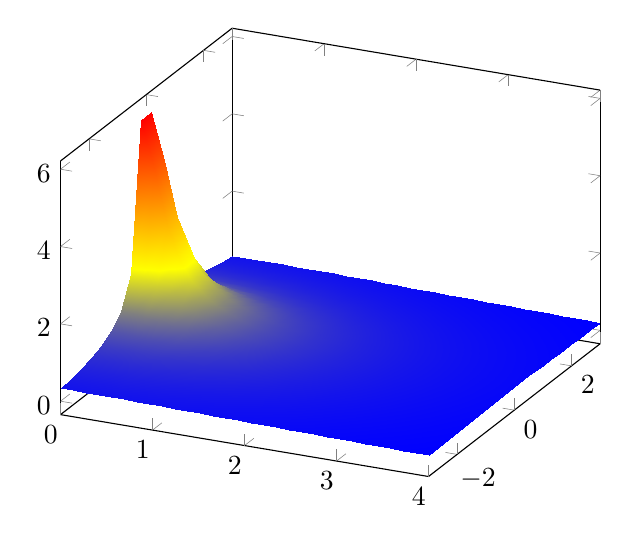
\begin{tikzpicture}
    \begin{axis}
      \addplot3 [
        domain=0:4,
        domain y = -3:3,
        samples = 30,
        samples y = 18,
        surf,
        % fill= yellow,
        shader = interp] {1/(sqrt(x^2+y^2))};
      % \addplot coordinates {(1,0,1)};
    \end{axis}
  \end{tikzpicture}
  \caption{We plot the absolute value of $ a_J $ with respect to real and imaginary part of $ J $.
    The orthogonality relation would only lead to the points corresponding to the positive integer values of $ J $.
    However, analyticity in $ J $ suggests that a more appropriate way to think about $ a_J $ is the whole colored manifold, rather than just the isolated points.
  }
  \label{fig:toyAnalyticity}
\end{figure}

\subsection*{Casimir equation}
Our goal is to introduce the Lorentzian inversion formula in a simple setting of two dimensions.
Most of the technical details are analogous in the generic dimensions.
We list the analogies with the toy model discussed above in \cref{ta:analogies}.

\begin{table}[ht ]
  \centering\begin{tabular}{c|c|c }
                                                                   & Toy model & CFT                                                      \\
    \hline
    Orthogonal partial wave                                        & $ w^{J} $ & $ F_{h + i \nu,J} \left( u,v \right) $                   \\
    Orthogonality relation                                         &
    $\oint \frac{dw}{2 \pi i} \, w^{J} w^{J'} = \delta_{-1-J,J'} $ &
    $ \int du \, dv \, \omega \, F_{h + i \nu,J}   \, F_{h + i \nu',J}  =\left(  n_{\nu,\nu'} \delta_{\nu,\nu'} + \text{shadow} \right) $ \\
    Coefficient function                                           & $ a_{J} $ & $ c_{\nu,J} $
  \end{tabular}
  \caption{Analogy between the toy model and the conformal field theories}
  \label{ta:analogies}
\end{table}

We summarize some useful properties of conformal blocks here \cite{Dolan:2003hv}.
The operator product expansion of two external operators can be arranged into families of operators such that all the operators are either a primary or its descendant
\begin{align}
  \phi \times \phi & = \sum_{O} \lambda_{O} O
  .\end{align}
This allows us to write the correlator as a sum over blocks with contribution coming from this primary
\begin{align}
  A \left( u,v \right) & = \sum_{O} \, \lambda_{O}^2 G_{O} \left( u,v \right)
  .\end{align}

However, we can use conformal symmetry to characterize the blocks in a different way.
Since they are functions of two variables $ u,v $, or alternatively, of $ z, \bar{z} $, they can be written as solutions to the differential equation, called the Casimir equation
\begin{align}
  C_2 \, G_{\Delta,J} & = c_2 \, G_{\Delta,J}
  .\end{align}
Here, we have used the notation that $ a = \left( \Delta_2 - \Delta_1 \right)/2 $ and $ b = \left( \Delta_3 - \Delta_4 \right)/2 $,
\begin{align}
  \label{eq:CasimirEq}
  C_2   & = D_z  + D_{\bar{z}} + \left( d-2 \right) \frac{z \bar{z}}{z - \bar{z}} \left[ \left( 1-z \right) \partial_{z} - \left( 1 - \bar{z} \right) \partial_{\bar{z}} \right] ,\nonumber \\
  c_2   & = \frac{1}{2} \left[ J\left( J+d-2 \right)+ \Delta\left( \Delta-d \right) \right]\nonumber                                                                                        \\
  D_{z} & = z^2 \partial_z \left( 1-z \right) \partial_z - \left( a+b \right)z^2 \partial_z -  a b z
  .\end{align}
For equal external scalars, these simplify due to $ a = b = 0 $.
The solutions to this equation admit several symmetries which they inherit from the Casimir eigenvalue, which correspond to swapping two elements in the following tuples,
\begin{align}
  \label{eq:swaps}
  \left( J \leftrightarrow 2-d-J \right),
  \quad
  \left( \Delta \leftrightarrow d-\Delta \right),
  \quad
  \left(\Delta  \leftrightarrow 1-J \right)
  .\end{align}

It can be seen that the differential equation in \cref{eq:CasimirEq} admits a power law solution in $ z , \bar{z} $ if we strip out a pure power law as a leading behavior.
Thus, we define a `pure' solution to the differential equation as the solution with the boundary condition
\begin{align}
  g_{\text{pure},\Delta,J}\left( z,\bar{z} \right) & =	z^{\frac{\Delta-J}{2}} \bar{z}^{\frac{\Delta + J}{2}} \left( 1 + \text{subleading power laws} \right)  \nonumber \\
                                                   & 0 \ll z \ll \bar{z} \ll 1
  .\end{align}
Thus, there are $ 8 $ solutions to the differential equation of the form $ g_{\text{pure},\Delta,J}$.
Each of which can be obtained by doing the swaps in \cref{eq:swaps} to the main pure solution $ g_{\text{pure},\Delta,J} $.
A general solution to the differential equation is a linear combination of these $ 8 $ solutions.

Two of the most important solutions are called the conformal block $ G_{\Delta,J} $ and the conformal partial wave $ F_{\Delta,J} $.
Conformal block resums the contribution of the primary and its descendant, whereas partial wave is a linear combination of the conformal block and its `shadow', $ \Delta \rightarrow d-\Delta $.
In two dimensions, the conformal block can be written in a closed form in terms of the hypergeometric functions
\begin{align}
  G_{\Delta,J } & = \frac{1}{1+\delta_{J,0}} \left[ k_{\Delta-J}\left( z \right) k_{\Delta+J}\left( \bar{z} \right) + k_{\Delta-J}\left( z \right)  k_{\Delta+J}\left( \bar{z} \right)  \right]
  .\end{align}
The two terms here are equivalent to $ g_{\text{pure}} $.
Here, we have defined
\begin{align}
  k_{\beta}^{a,b}\left( z \right) & = z^{\beta/2}
  {{}_{2}F_{1}\left(\genfrac..{0pt}{}{\beta/2+ a , \beta/2 +b}{\beta};z\right)}
  .\end{align}
The conformal blocks in general dimensions can be written in a similar fashion.
We use the shorthand $ g $ to denote $ g_{\text{pure}} $.
\begin{align}
  G_{\Delta,J} & = g_{\Delta,J} + \frac{\Gamma\left( J+d-2 \right)  \Gamma\left( -J - \frac{d-2}{2} \right)	}{ \Gamma\left( J+ \frac{d-2}{2} \right) \Gamma\left( -J \right)}  g_{\Delta, 2-d-J}
  .\end{align}

A more useful object for our purpose is the conformal partial wave, $ F_{\Delta,J} $, as it admits nice orthogonality properties.
It is defined as the unique linear combination of the conformal block, $ G_{\Delta, J} $, and its shadow, $ G_{d-\Delta, J} $, that is single valued in the Euclidean signature.
Here, Euclidean signature means $ \bar{z} = z^{*} $,
\begin{align}
  \label{eq:partialWaveIntro}
  F_{\Delta,J} & =\frac{1}{2}\left[  G_{\Delta,J} + \frac{K_{d-\Delta,J} }{K_{\Delta,J} }G_{\Delta,J} \right]
  .\end{align}
We suppress the definition of $ K $ and refer to \cite{Caron-Huot:2017vep}, for the definitions of $ K $.

Alternatively, these can be thought of as the solutions of the Sturm-Liouville problem defined by the Casimir equation.
In particular, they admit an orthogonality property for the scaling dimensions $ \Delta = d/2 + i \nu $ when $ \nu $ is a real number \cite{Caron-Huot:2017vep},
\begin{align}
  I_{J,\nu, J',\nu'} & =
  \int d^2z \, \mu\left( z,\bar{z} \right) F_{\frac{d}{2}  + i \nu,J}  F_{\frac{d}{2}  + i \nu',J'}
  .\end{align}
Here, $ I_{J,\nu, J',\nu'} $ acts as a delta function along with some normalization factor, $ n $.
One needs to use the properties of the Gegenbauer polynomials, the spherical polynomials in $ d $ dimensions, in order to show the orthogonality property.

It can be used to write the Euclidean inversion formula, as follows,
\begin{align}
  \label{eq:EuclideanInversionIntro}
  c_{\Delta,J} & = n_{\Delta,J} \int d^2z \, \mu\left( z,\bar{z} \right) F_{\Delta,J} \left( z,\bar{z} \right) A\left( z,\bar{z} \right)
  .\end{align}
This can be rewritten in a useful way in terms of $ \sigma  = \sqrt{z \bar{z}}$ and $ w = \text{exp} \left( i \arccos \left( \xi \right)  \right) $.
We remind that the angle
\begin{align}
  \xi & =	\frac{1}{2} \left(
  \sqrt{\frac{z}{\bar{z}}} + \sqrt{\frac{\bar{z}}{z}}
  \right)
  ,\end{align}
and $ w $ is a phase factor associated with it.
The integral over the Euclidean region can be recast as an integral over $ \sigma $ in $ \left( 0,1 \right) $ and $ w $ on a unit circle.
This is shown as the blue contour in the \cref{fig:wcontourdeformatoinInversionFormula}.
This is analogous to the orthogonality relation of the power laws in the toy model presented above.
Now, we move to the contour deformation of this blue contour.

In order to do this, we need to discuss the behavior of the pure blocks when we analytically continue them away from the Euclidean region.
This can be done by studying the analytic structure of the lightcone limit of these blocks, $ 0 \ll z \ll \bar{z}  $ without taking any limit for $ \bar{z} $.
In this limit,
\begin{align}
  g_{\Delta,J} & \rightarrow z^{\frac{\Delta-J}{2}} k_{\Delta+J}\left( \bar{z} \right)
  .\end{align}
Since the analytic continuations happen in $ \bar{z} $ around $ 1 $, we would like to know the monodromy of this function around around $ 1 $.
We note a useful identity,
\begin{align}
  \, _2F_1(a,b;c;z) & =\frac{\Gamma (c) (1-z)^{-a-b+c} \Gamma (a+b-c) }{\Gamma (a) \Gamma (b)}
  \,
  _2F_1(c-a,c-b;-a-b+c+1;1-z) \nonumber                                                        \\
                    & +\frac{\Gamma
    (c) \Gamma (-a-b+c) }{\Gamma (c-a) \Gamma
    (c-b)}\, _2F_1(a,b;a+b-c+1;1-z)
  .\end{align}
This can be used to map the nontrivial monodromy at $ \bar{z} = 1 $ to monodromy of the power laws at $ \bar{z} = 0 $.
As a result, one can show that, for some functions $ \alpha $ and $ \beta $ of the operator data $ \Delta,J $
\begin{align}
  \label{eq:analyticContinuationOfgpure}
  g^{\circlearrowleft}_{\Delta,J}\left( z,\bar{z} \right) & = \alpha_{\Delta,J} g_{\Delta,J}\left( z,\bar{z} \right) + \beta_{\Delta,J} g_{1-J,1-\Delta} \left( z,\bar{z} \right)
  .\end{align}
Similar formula can be written for $ g^{\circlearrowright} $.
As any solution to the Casimir equation can be written as a linear combination of these $ g_{\Delta,J} $, we can deduce the analytic continuation of any such solution along any path in the complex $ \bar{z} $ plane.




\begin{figure}[t!]
  \centering

  \resizebox{0.6\textwidth}{!}{
    \begin{tikzpicture}
      %name
      \draw[] (-2.2,3) -- (-2.2,2.5) -- (-2.7,2.5);
      \node[left] at (-2.2,2.8) {$w$};
      \node[below right] at (1,0) {$1$};
      \node[below right] at (2,0) {$\frac{1}{\sigma}$};
      \node[above] at (0.5,0) {$\sigma$};
      \node[below left] at (-1,0) {$-1$};
      \node[below left] at (-2,0) {$-\frac{1}{\sigma}$};
      \node[above] at (-0.5,0) {$-\sigma$};
      % \node[below] at (0,0) {$0$};
      % \node[below right] at (3,0) {$\infty$};
      %axis
      \draw[->,opacity=0.3,-latex'] (0,0) -- (-3.5,0);
      \draw[->,opacity=0.3,-latex'] (0,0) -- (0,3.5);
      \draw[->,opacity=0.3,-latex'] (0,0) -- (0,-3.5);
      \draw[->,opacity=0.3,-latex'] (0,0) -- (3.5,0);
      %circle
      \draw[blue,dashed] (0,0) circle (1);

      \draw[red,fill= red,dashed] (0,0) circle (0.05);
      \draw[red,fill= red,dashed] (1,0) circle (0.05);
      \draw[red,fill= red,dashed] (2,0) circle (0.05);
      \draw[red,fill= red,dashed] (-1,0) circle (0.05);
      \draw[red,fill= red,dashed] (-2,0) circle (0.05);
      \draw[red,fill= red,dashed] (-1/2,0) circle (0.05);
      \draw[red,fill= red,dashed] (1/2,0) circle (0.05);
      %red
      \draw[red, thick] (-3,0) -- (3,0);
      \draw[red,dashed] (0,0) circle (3);
      \draw[red,dashed] (-3,0.05) -- (3,0.05);
      \draw[red,dashed] (-3,-0.05) -- (3,-0.05);
      % \draw (5,0) arc(5:175:5) ;
      \node[below] at (2,2) {$C_{+}$};
      \node[above] at (2,-2) {$ C_{-}$};
    \end{tikzpicture}
  }
  \caption{Contour deformation in the inversion formula. Blue contour corresponds to the Euclidean inversion formula. The cuts lie at the whole real axis for various branch points shown in red.
    Dashed red contour corresponds to the Lorentzian formula.
  }
  \label{fig:wcontourdeformatoinInversionFormula}
\end{figure}

\subsection*{Lorentzian formula}

% \textbf{Add rest of the derivation }
In the toy model, we used Cauchy formula to deform the contour to arrive at a novel representation of the coefficient function that displays the nice analyticity properties.
We would like to use the same idea for the Euclidean inversion formula.
We outline the key steps involved in the derivation.

We would like to analyze the cut structure of the correlation as well as the weight of the orthogonality relation.
The branch points corresponding to those nontrivial analytic behaviors are plotted in \cref{fig:wcontourdeformatoinInversionFormula}.
For the purpose of this section, we will use the cross ratios $ \rho, \bar{\rho} $:
\begin{align}
  \rho = \frac{
    1 - \sqrt{1- z}
  }{
    1 + \sqrt{1- z}
  },
   &  &
  \bar{\rho} = \frac{
    1 - \sqrt{1- \bar{z}}
  }{
    1 + \sqrt{1- \bar{z}}
  }
  .\end{align}
In the Lorentzian setup, they become lightcone coordinates as shown in \cref{fig:ReggeFigLightcones}.
To make contact with toy model, it is useful to change the variables further to
\begin{align}
  \rho = \sigma w, &  & \bar{\rho} = \frac{\sigma }{w}
  .\end{align}
These are precisely the variables used in the \cref{eq:EuclideanInversion}.
We will use these variables to rewrite the Euclidean inversion formula \cref{eq:EuclideanInversion} as
\begin{align}
  c_{\Delta,J}
   & = n_{\Delta,J}
  \displaystyle\int_{0}^{1} \, \sigma \, d \sigma  \oint \frac{dw}{i\, w }
  \, \mu\left( \rho,\bar{\rho} \right)
  A\left( \rho, \bar{\rho} \right)  F_{\Delta,J} \left( \rho, \bar{\rho} \right)
  .\end{align}
The contour for $ w $ is shown in red in the \cref{fig:wcontourdeformatoinInversionFormula}.
The branch points corresponds to the lightcones as well as the branch points of the weight function.

We would deform this contour in two ways.
First, we split the integrand according to the part which diverges at $ w = 0 $ and the part which does not.
Then, for the part that converges at $ w = 0 $, we deform the contour inward, whereas for the other part we deform the contour outward.
This will result in two contours as shown in \cref{fig:wcontourdeformatoinInversionFormula}.
Individually, these contour contribute $ 0 $, since the function inside them is analytic.

Note that, we have also made an assumption to drop the arcs at $ \infty $ and at $ 0 $.
This is the assumption of boundedness in the Regge limit.


\begin{figure}[tbp]
  \centering
  \resizebox{0.8\textwidth}{!}{
    \begin{tikzpicture}
      %draw a square with points at (2,0) (0,2) (0,-2) (-2,-2)
      % \draw[thick] (4,0) -- (0,4)  -- (-4,0) -- (0,-4)-- cycle;
      %draw side bisectors
      \draw[dashed,opacity=0.4] (2,2) -- (-2,-2);
      \draw[dashed,opacity=0.4,red] (0.5,2) -- (-1.5,0);
      \draw[dashed,opacity=0.4,red] (-0.5,-2) -- (1.5,0);
      \draw[dashed,opacity=0.4] (2,-2) -- (-2,2);
      %points
      % \node[below] at (0.7,0) {$5$};
      % \draw[fill,black](0.7,0) circle (0.05cm);
      \node[right] at (1.5,0) {$1:(1,1)$};
      \draw[fill,black](1.5,0) circle (0.05cm);
      \node[right] at (2,-1.8) {$3$};
      \draw[fill,black](2,-1.8) circle (0.05cm);
      % \node[below] at (2,-2.2) {$4^{-}$};
      % \draw[fill,gray,opacity=0.4](2,-2.2) circle (0.05cm);
      \node[left] at (-1.5,0) {$2:(-1,-1)$};
      \draw[fill,black](-1.5,0) circle (0.05cm);
      % \node[above] at (2,2.2) {$2^{+}$};
      % \draw[fill,gray,opacity=0.4](2,2.2) circle (0.05cm);
      \node[left] at (-2,1.8) {$4$};
      \draw[fill,black](-2,1.8) circle (0.05cm);

      %arrows for Regge 
      \draw[->,opacity=0.4,-latex',thick] (0.2,0) -- (2,-1.8);
      \draw[->,opacity=0.4,-latex',thick] (-0.2,0) -- (-2,1.8);
      % \draw[->,opacity=0.4,-latex'] (1.6,1.1) to[out=90,in=225] (2,1.7);
      % \draw[->,opacity=0.4,-latex'] (-1.6,1.1) to[out=90,in=-45] (-1.9,1.7);
      % \draw[->,opacity=0.4,-latex'] (1.6,-1.1) to[out=270,in=135] (1.9,-1.7);
      % \draw[->,opacity=0.4,-latex'] (-1.6,-1.1) to[out=270,in=45] (-1.9,-1.7);

      %plot axis and label
      \draw[-stealth] (4.9,0) -- (5.4,0.5) node[anchor=south,right]{$ \bar{\rho} $ };
      \draw[-stealth] (4.9,0) -- (5.4,-0.5) node[anchor=south,right]{$ \rho $ };
    \end{tikzpicture}
  }
  \caption{Regge limit configuration in the Lorentzian cylinder.
    The red lines correspond to the lightcones crossed by the points $ 3 $ and $ 4 $.
  }
  \label{fig:ReggeFigLightcones}
\end{figure}

In practice, we do these contour manipulations using the ideas from representation theory of the conformal group.
The most general solution to Casimir equation is represented by $ 8 $ functions with various weights $ g_{\Delta,J} $.
They can be simple understood as the values of $ \Delta, J  $ such that the Casimir eigenvalue $ C_2 = \Delta \left( \Delta-d \right) + J\left( J+d-2 \right)  $ remains unchanged.
Again, the contour integral over $ C_{\pm} $ is $ 0 $ for all of them.

The count of $ 8 $ can be achieved from the analytic continuation of the conformal partial waves, as follows.
The conformal partial wave $ F_{ \Delta, J } $ is already a sum of two conformal blocks, $ G_{\Delta,J} $ functions, as shown in \cref{eq:partialWave}.
Each of the blocks is a sum of two $ g_{\Delta,J} $ functions.
However, after analytic continuation, each of the $ g_{\Delta,J} $ functions picks monodromy which contains yet another $ g_{\Delta,J} $ function, as shown in \cref{eq:analyticContinuationOfgpure}.

The analytic continuation can be done using these formulae.
Since we have dropped the arcs at $ \infty $, we arrive at only an integral over the real axis with small positive or negative imaginary part, for $ C_{\pm} $.
By splitting these integrals into intervals separated by the various branch points on the real axis $ \sigma, 1 , 1/\sigma,-\sigma, -1 , -1/\sigma $, we get several integrals over the ranges such as $ w \in \left( 0,1/\sigma \right) $.
The cuts with $ w>0 $ and $ w < 0 $ are treated separately.
The contributions from the four regions with $ w>0 $ combie to give a $ \dDisc \left( A \right) $.
The regions with negative $ w $ give rise to the integral that is the same as the positive $ w $ region, but with an extra factor of $ \left( -1 \right)^J $.
The final formula for $ c_{\Delta,J} = c^{t}_{\Delta,J} + c^{u}_{\Delta,J} $ in terms of $ z,\bar{z} $ looks as follows \cite{Caron-Huot:2017vep},
\begin{align}
  c^{t}_{\Delta,J} & = \frac{\kappa_{\Delta+J}}{4} \int_{0}^{1} dz \, d\bar{z} \, \mu\left( z, \bar{z} \right) G_{J+d-1,\Delta+1-d}\left( z,\bar{z} \right) \dDisc\left[ A \left( z, \bar{z} \right) \right]
  .
\end{align}





The main implication of the analyticity property is to show the rigidity in the spectrum of the conformal field theories.
The claim of analyticity is not just an abstract mathematical statement, but can be seen at weak coupling theories as in \cref{fig:3dintercept}.
Analyticity is also useful in justifying the large spin expansion of the CFT data.
A priori, such an expansion of the CFT data is only asymptotic.
However, analyticity in $ J $ shows that for $ \text{Re } J >1$, the coefficient function is analytic.
Therefore, it can be expanded around $ J = \infty $ to yield a convergent series \cite{Simmons-Duffin:2016wlq}.
This can be checked with the analysis from the numerical bootstrap as shown in the \cref{fig:DSDLightcone}.



\begin{figure}[tb]
  \begin{center}
    \includegraphics[scale=.5]{Figures/3dIntercept.pdf}
    \caption{The figure taken from \cite{Caron-Huot:2022eqs}. An $\mathbb{R}^3$ projection of the $\mathbb{C}^2$ Chew-Frautschi plot of the leading Regge trajectory in Wilson-Fisher theory near the intercept at $O(\e^4)$.  The imaginary part of $J$ is shown by color, with negative values in blue and positive values in red. Even though the two branches appear to intersect, they do not -- in order to intersect in $\mathbb{C}^2$, they need to intersect in this $\mathbb{R}^3$ projection and also have the same color.  The plot is made at $\e=0.3$.}
    \label{fig:3dintercept}
  \end{center}
\end{figure}

\begin{figure}[t!]
  \centering
  \includegraphics[width=0.8\textwidth]{Figures/tauSigSig0.pdf}
  \caption{Results from the numerical analysis \cite{Simmons-Duffin:2016wlq}.
    It depicts the spectrum of operators in the operator product expansion of $ \sigma \times \sigma $.
    To facilitate the comparison with analytic result, the vertical axis plots $  \tau= \Delta- J $, `twist' and $ \bar{h} = \frac{\Delta + J}{2} $.
    Notice the present of stress-tensor with $ \Delta = 3 , \tau = 1$.
    The continuous line is the extrapolation of the large spin perturbation theory around $ J = \infty $.
    While the spin $ J = \bar{h} - h  $ is as small as $ 2 $, we find a remarkable agreement with the numerics.
  }
  \label{fig:DSDLightcone}
\end{figure}
\section{Plan of the thesis}
The discussion of the analyticity in spin sets the stage for the thesis.
The goal of the thesis is to consider two aspects of Regge theory.
\subsection*{Optical theorem in AdS}
In recent years it has been shown that powerful analytical results for scattering amplitudes in quantum field theory, namely the Froissart-Gribov formula and dispersion relations, have equally powerful CFT analogues in the Lorentzian inversion formula \cite{Caron-Huot:2017vep,Karateev:2018oml,Kravchuk:2018htv,Lemos:2017vnx,Liendo:2019jpu} and the two-variable CFT dispersion relation \cite{Carmi:2019cub,Caron-Huot:2020adz}. Dispersion relations reconstruct a scattering amplitude from the discontinuity of the amplitude, while the Froissart-Gribov formula extracts the partial wave coefficients from the discontinuity and makes their analyticity in spin manifest. The utility of these methods as computational tools for scattering amplitudes stems from the fact that the discontinuity of an amplitude (or that of its integrand) in perturbation theory is determined in terms of lower-loop data by the optical theorem, which in turn is a direct consequence of unitarity.
The CFT analogue of the discontinuities of amplitudes, which contain the dispersive data and are of central importance in the aforementioned analytical results, is the double discontinuity (dDisc) of CFT four-point functions. The Lorentzian inversion formula
computes OPE data (anomalous dimensions and OPE coefficients) from the dDisc of four-point functions and establishes the analyticity in spin of OPE data. The CFT dispersion relation, much like its QFT inspiration, directly reconstructs the full correlator from the dDisc. There also exist simpler single-variable dispersion relations in terms of a single discontinuity (Disc) of the correlation function that determine only the OPE coefficients while the anomalous dimensions are required as inputs \cite{Bissi:2019kkx}.

The unitarity based methods to compute amplitudes  inspire the development of  similar unitarity methods for CFT, in particular,
for the dDisc of four-point functions one gains a loop or leg order for free.
It was first noticed in large spin expansions \cite{Alday:2016njk,Alday:2016jfr,Aharony:2016dwx} and later understood more generally in terms of the Lorentzian inversion formula
that OPE data at one-loop can be obtained from tree-level data \cite{Alday:2017vkk,Alday:2017zzv}. Generically, in perturbative CFT calculations the dDisc at a given order only depends on OPE data from lower order or lower-point correlators. More recently, in the context of the AdS/CFT correspondence \cite{Maldacena:1997re,Witten:1998qj,Gubser:1998bc},
these unitarity methods for CFT have been related to cutting rules for computing the dDisc of one-loop Witten diagrams \cite{Liu:2018jhs} from tree-level diagrams \cite{Ponomarev:2019ofr,Meltzer:2019nbs,Meltzer:2020qbr}.
See also the earlier work of \cite{Fitzpatrick:2011dm}.

However, so far we have been missing a direct adaptation of the optical theorem to CFT correlation functions.
More concretely, we lacked the ability to express the dDisc of a perturbative correlator, at a given order in the perturbative parameter, in terms of lower order correlators, without the detour via the OPE data and without making explicit reference to AdS Witten diagrams.
In the first chapter, we provide a direct CFT derivation of such unitarity relations.
In particular, we present an optical theorem for 1-loop four-point functions wherein the dDisc is fixed in terms of single discontinuities of lower-loop  correlators.

\subsection*{Conformal multi-Regge theory}

Constraints from the bootstrap analysis of the four point correlation functions are known to be powerful in obtaining remarkable accurate and precise physical data such as critical exponents of the theories appearing in the nature.
The main idea is that any function of two cross ratios can not  be a valid correlation function.

This suggests that there might be more constraints in the consistency of higher point correlation functions.
Since higher point functions can be decomposed into correlation functions with fewer number of points, these constraints are implicitly present in the four point bootstrap analysis.
However, we might need to explore \emph{infinitely} many four point functions to probe them.
For instance, a single five point correlation function can be decomposed into infinitely many four point functions.
This calls for a careful study of such high point functions.

In the third chapter, our goal is to initiate such a program.
The goal is to introduce a useful definition of Regge limit for five point correlation functions in conformal field theories.
First, we review the relevant literature from S-matrix theory.
In particular, we discuss the multi-Regge limit of five point string theory amplitudes.

Inspired by this analysis, we propose the generalization to the conformal field theory.
Since the natural analogue of the Mandelstam invariants is the Mellin space, we discuss this generalization mainly in Mellin space.
We also show its relation to position space and the corresponding spacetime structure.

Furthermore, we comment on the relation between the Reggeized correlator and the CFT data such as the OPE coefficients and the scaling dimensions of the operators on the leading Regge trajectory.
In passing, we also discuss several interesting kinematical aspects of higher point correlation functions.
We expect them to be useful in generalizing the discussion of the inversion formula and the dispersion relation to the higher point functions.

Now, we turn to the analysis of the optical theorem in $ AdS $.
\cleardoublepage
